\documentclass[tikz,border=5mm]{standalone}
\usepackage{pgfplots}
\usepackage{amsmath}
\pgfplotsset{compat=1.18}

\begin{document}
	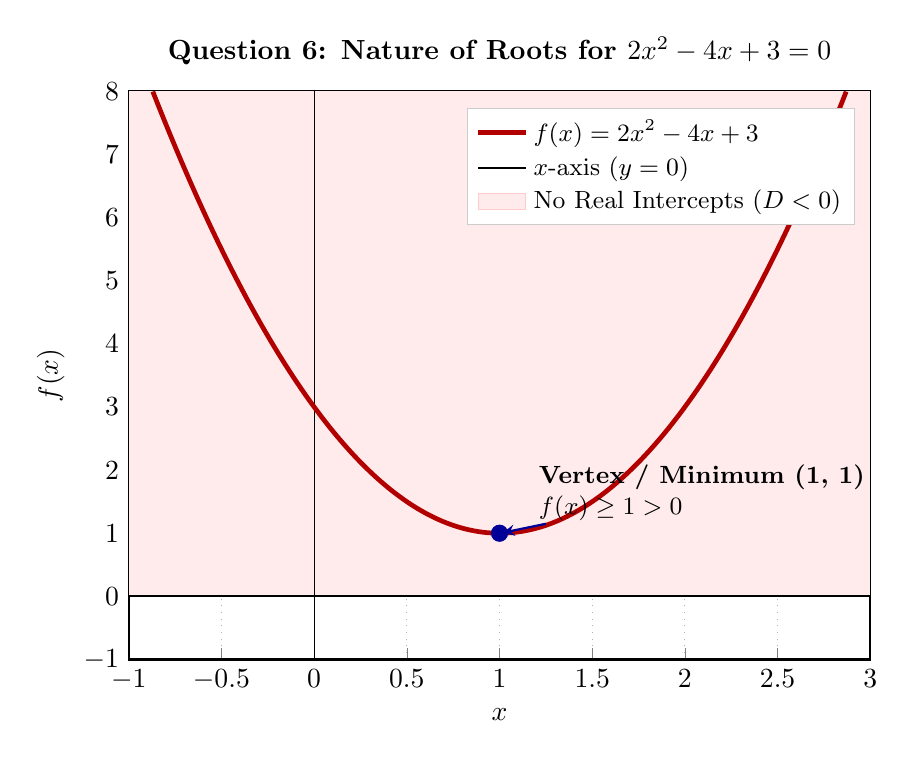
\begin{tikzpicture}
		\begin{axis}[
			width=11cm, height=8.8cm,
			title={\textbf{Question 6: Nature of Roots for $2x^2 - 4x + 3 = 0$}},
			xlabel={$x$}, ylabel={$f(x)$},
			xmin=-1.0, xmax=3.0,
			ymin=-1.0, ymax=8.0,
			xtick={-1.0,-0.5,0.0,0.5,1.0,1.5,2.0,2.5,3.0},
			xticklabel style={/pgf/number format/fixed, /pgf/number format/precision=1},
			ytick={-1,0,1,2,3,4,5,6,7,8},
			grid=both,
			grid style={dotted, gray!60},
			axis line style={black, thick},
			legend cell align={left},
			legend style={at={(0.98,0.97)}, anchor=north east, font=\small, draw=gray!40}
			]
			% Pale red shaded region for y >= 0
			\fill[fill=red!8] (axis cs:-1,0) rectangle (axis cs:3,8);
			
			% Axis lines
			\draw[black, thin] (axis cs:0,-1) -- (axis cs:0,8);
			\draw[black, thick] (axis cs:-1,0) -- (axis cs:3,0);
			
			% Parabola f(x) = 2x^2 - 4x + 3
			\addplot[domain=-0.87:2.87, samples=150, color=red!70!black!, line width=1.7pt] {2*x^2 - 4*x + 3};
			\addlegendentry{$f(x) = 2x^2 - 4x + 3$}
			
			% x-axis entry for legend
			\addplot[black, thick] coordinates {(-1,0) (-1,0)};
			\addlegendentry{$x$-axis ($y = 0$)}
			
			% Fill legend entry
			\addlegendimage{area legend, fill=red!8, draw=red!20}
			\addlegendentry{No Real Intercepts ($D < 0$)}
			
			% Vertex dot
			\node[circle, fill=blue!60!black, inner sep=2.2pt] at (axis cs:1,1) {};
			
			% Vertex Annotation with arrow
			\draw[<-, >=stealth, thick, blue!60!black] (axis cs:1.02, 1.01) -- (axis cs:1.25, 1.15);
			\node[anchor=south west, font=\small, inner sep=0pt] at (axis cs:1.12, 1.15) {
				\begin{tabular}{l}
					\textbf{Vertex / Minimum (1, 1)} \\
					$f(x) \ge 1 > 0$
				\end{tabular}
			};
		\end{axis}
	\end{tikzpicture}
\end{document}